\section{\texorpdfstring{$L^2$}{L2}空间}
\label{sec:ipspace-l2-space}

上一节的两个不完备例子分别缺少平方可和的数列和平方可积的阶跃函数。第~\ref{chap:function-normed-spaces}章已经在几乎处处等价类上建立了$L^2$，并证明它在$L^2$范数下完备。接下来只需在$L^2$上定义内积，并核对它诱导的正是这个范数。本节固定测度空间$(X,\mathcal A,\mu)$。

\paragraph{\texorpdfstring{$L^2$}{L2}内积}
点积推广到函数时写成乘积的积分，首先要保证这个积分有意义。有限维的和总是有限的，无限维时要靠条件。对$f,g\in L^2(\mu)$，Hölder不等式在$p=q=2$时给出
\[
 \int_X\lvert\bar fg\rvert\,d\mu=\int_X\lvert f\rvert\,\lvert g\rvert\,d\mu\leq\lVert f\rVert_2\,\lVert g\rVert_2<\infty,
\]
所以$\bar fg$可积。

于是可以令
\begin{equation}
 \langle f,g\rangle=\int_X\bar fg\,d\mu ,
 \label{eq:ipspace-l2-inner-product}
\end{equation}
实函数时共轭可以省去。复值函数的积分按第~\ref{chap:integration}章的规定，实部、虚部分别积分。

这个定义不依赖代表的选择。若$f'\sim_\mu f$、$g'\sim_\mu g$，则$\bar f'g'$与$\bar fg$只在零测集$\{f'\neq f\}\cup\{g'\neq g\}$上可能不同，积分相同。所以$\langle\cdot,\cdot\rangle$是等价类上定义合理的映射。

\paragraph{内积公理与诱导范数}
对第二个变量的线性来自积分的线性，共轭对称来自$\overline{\int\bar fg\,d\mu}=\int f\bar g\,d\mu$。正定性值得细看：被积函数非负，所以
\[
 \langle f,f\rangle=\int_X\lvert f\rvert^2\,d\mu\geq0 ,
\]
且它为零当且仅当$\lvert f\rvert^2=0$几乎处处，也就是$[f]$是零元素。

正是等价类使正定性成立。若在普通函数上计算，只在一点非零的函数也会使$\langle f,f\rangle=0$，正定性就失败了。第~\ref{sec:ipspace-inner-products}节说过，积分内积中单个点没有权重；把函数换成等价类，就是承认这件事，不再区分只差一个零测集的函数。

诱导范数是
\[
 \sqrt{\langle f,f\rangle}=\Bigl(\int_X\lvert f\rvert^2\,d\mu\Bigr)^{1/2}=\lVert f\rVert_2 ,
\]
恰好是第~\ref{chap:function-normed-spaces}章的$L^2$范数。那里已经证明$L^2(\mu)$在这个范数下完备，所以下面的定理不需要新的论证。

\begin{theorem}[$L^2$是Hilbert空间]
\label{thm:ipspace-l2-hilbert}
对任意测度空间，$L^2(\mu)$配以式~\eqref{eq:ipspace-l2-inner-product}的内积是Hilbert空间。
\end{theorem}

上一节的阶跃例子在这里有了去处。$\operatorname{sgn}$的等价类属于$L^2[-1,1]$。$g_n$与$\operatorname{sgn}$只在$\lvert x\rvert<1/n$上不同，左右两半对称，所以
\[
 \lVert g_n-\operatorname{sgn}\rVert_2^2=2\int_0^{1/n}(1-nx)^2\,dx=\frac{2}{3n}\to0 .
\]
斜坡列在$L^2[-1,1]$中收敛到$\operatorname{sgn}$。

\paragraph{\texorpdfstring{$\ell^2$}{l2}空间}
取$X=\mathbb N_+$与计数测度，积分变成求和，等价类就是数列本身，得到
\begin{equation}
 \begin{gathered}
 \ell^2=\Bigl\{x=(x_k):\ \sum_{k\geq1}\lvert x_k\rvert^2<\infty\Bigr\},\\
 \langle x,y\rangle=\sum_{k\geq1}\overline{x_k}\,y_k .
 \end{gathered}
 \label{eq:ipspace-ell2}
\end{equation}
这是最字面意义上的“无限维向量空间”：元素就是$[a_1,a_2,\ldots]$，内积就是点积，唯一的新要求是长度有限。级数的绝对收敛来自计数测度下的Hölder不等式。由定理~\ref{thm:ipspace-l2-hilbert}，$\ell^2$是Hilbert空间。

$c_{00}$是$\ell^2$的子空间，内积是限制后的内积，上一节的柯西列$x^{(N)}$在$\ell^2$中收敛到$(1/k)$。$c_{00}$的不完备，只是因为它没有包含这些极限。有限维的$\mathbb K^d$可以看作只有前$d$项非零的数列，这时$\ell^2$内积就是卷二的标准内积。

$\ell^2$与$L^2[-1,1]$的差别值得留意。两者都是Hilbert空间，但$\ell^2$的下标是离散的，每个坐标都带着权重$1$，读取第$k$个坐标是连续的操作；$L^2[-1,1]$中单点没有权重，读取函数在某一点的值根本没有定义。

\paragraph{\texorpdfstring{$L^2$}{L2}中的正交}
函数的正交是乘积的积分为零。图~\ref{fig:ipspace-integral-orthogonality}在$L^2[-1,1]$中对照了两种情形：$1\cdot x$在正负半区间上的带符号面积相互抵消；$1\cdot x^2$处处非负，面积无处抵消。同样的对称性说明，$[-1,1]$上任何偶函数都与任何奇函数正交，因为乘积是奇函数，积分为零。

\begin{BookInlineFigure}
  \centering
  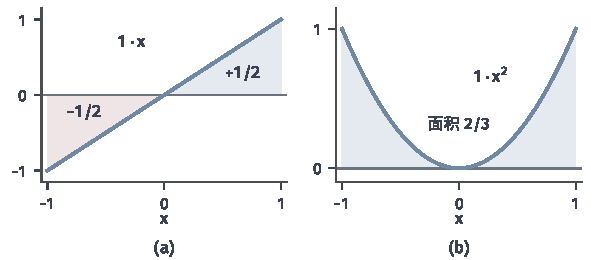
\includegraphics[width=100mm]{figures/04-spaces-measures-and-geometry/03-function-spaces/matplotlib/ipspace-integral-orthogonality/figure.pdf}
  \caption{积分内积下的正交。$[-1,1]$上取Lebesgue测度，曲线是两个函数的乘积，阴影是带符号面积。(a)$1\cdot x$的正负面积各为$\tfrac12$，内积为$0$，$1$与$x$正交。(b)$1\cdot x^2$处处非负，内积为$\tfrac23$，$1$与$x^2$不正交。}
  \label{fig:ipspace-integral-orthogonality}
\end{BookInlineFigure}

复情形的典型例子是复指数。在$L^2[-\pi,\pi]$中，对整数$j,k$，第一个变量取共轭，指数相减：
\[
 \begin{aligned}
 \langle e^{\mathrm ijx},e^{\mathrm ikx}\rangle
 &=\int_{-\pi}^{\pi}e^{-\mathrm ijx}e^{\mathrm ikx}\,dx\\
 &=\int_{-\pi}^{\pi}e^{\mathrm i(k-j)x}\,dx .
 \end{aligned}
\]
当$j=k$时被积函数为$1$，积分为$2\pi$。当$j\neq k$时，$e^{\mathrm imx}$（$m=k-j\neq0$）在一个周期上积分为零，因为它的原函数$e^{\mathrm imx}/(\mathrm im)$在两端取值相同。

所以$\{e^{\mathrm ikx}/\sqrt{2\pi}\}_{k\in\mathbb Z}$两两正交且长度为$1$。这一族是否足以表示$L^2[-\pi,\pi]$的每个元素，是第~\ref{chap:fourier-transform}章的问题。
